\documentclass[dvipsnames,border=3pt]{standalone}
\usepackage{tikz}
\usetikzlibrary{arrows}
\usetikzlibrary{shapes}
\usepackage{enumitem}
\usepackage{bm}
\usepackage{mathdots}
\usepackage{amsmath}
\usetikzlibrary{shadings}
\usetikzlibrary{decorations.pathreplacing}
\usepackage{helvet}
\usetikzlibrary{arrows.meta}
\usepackage{graphicx}
\usepackage{pgfplots}
\usepackage{pgfplotstable}
\usepackage{filecontents}
\usetikzlibrary{plotmarks}
\pgfplotsset{compat=newest}
\usepackage{xcolor}

\renewcommand{\familydefault}{\sfdefault}

\definecolor{mylightgray}{cmyk}{0,0,0,0.1}
\usetikzlibrary{arrows,decorations.pathmorphing,backgrounds,fit,positioning,shapes.symbols,chains}

\begin{document}

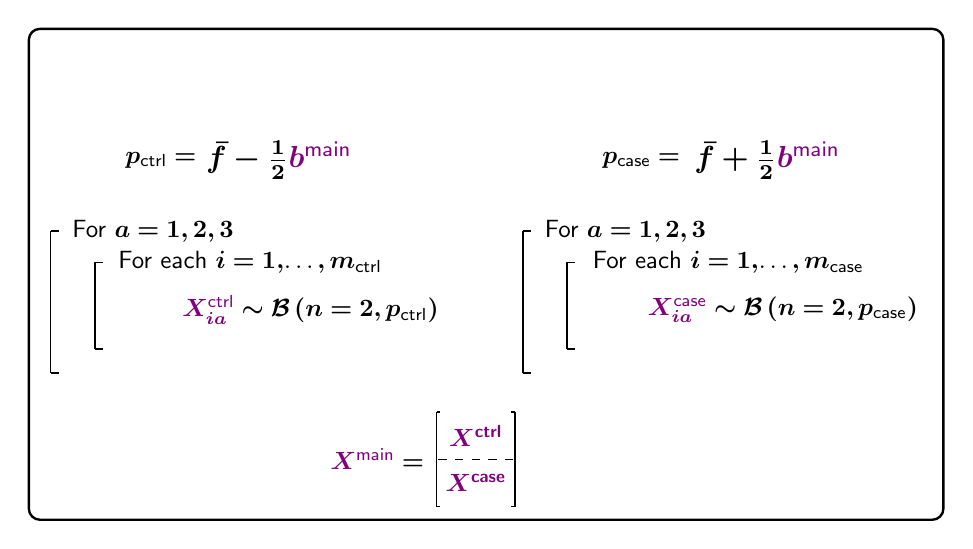
\begin{tikzpicture}
    % trim=left botm right top
    
    \node[draw, rounded corners=4, line width=0.3mm, text width=11.38cm, text height=6cm] at (12.23,-9.75) {};
    %\node[circle,draw,line width=0.2mm,xscale=1.2,yscale=1.2,fill=GreenYellow] at (7,-7.6) {};
    %\node at (7,-7.6) {\textbf{5}};
    
    % controls
    \node[xscale=0.9,yscale=0.9] at (8.1,-8.3) {\bm{$p_\text{ctrl}= $}};
    \node[xscale=1.1,yscale=1.1] at (9.6,-8.3) {\bm{$\bar{f} - \frac{1}{2}\textcolor{violet}{b^\text{main}}$}};
    
    \node[xscale=0.9,yscale=0.9] at (8,-9.2) {For \bm{$a = 1, 2, 3$}};
    \node[xscale=0.9,yscale=0.9] at (9.235,-9.6) {For each \bm{$i=1,$}$\dots$\bm{$,m_\text{ctrl}$}};
    
    \node[xscale=0.9,yscale=0.9] at (10,-10.2) {\bm{$\textcolor{violet}{X^\text{ctrl}_{ia}} \sim \mathcal{B}\left(n=2,p_\text{ctrl}\right)$}};
    
    \draw[line width=0.2mm] (6.7,-9.2) -- (6.7,-11);
    \draw[line width=0.2mm] (6.7,-9.2) -- (6.8,-9.2);
    \draw[line width=0.2mm] (6.7,-11) -- (6.8,-11);
    
    \draw[line width=0.2mm] (7.26,-9.6) -- (7.26,-10.7);
    \draw[line width=0.2mm] (7.26,-9.6) -- (7.36,-9.6);
    \draw[line width=0.2mm] (7.26,-10.7) -- (7.36,-10.7);
    
    % cases
    \node[xscale=0.9,yscale=0.9] at (14.2,-8.3) {\bm{$p_\text{case}=$}};
    \node[xscale=1.1,yscale=1.1] at (15.8,-8.3) {\bm{$\bar{f} + \frac{1}{2}\textcolor{violet}{b^\text{main}}$}};
    
    \node[xscale=0.9,yscale=0.9] at (14,-9.2) {For \bm{$a = 1, 2, 3$}};
    \node[xscale=0.9,yscale=0.9] at (15.305,-9.6) {For each \bm{$i=1,$}$\dots$\bm{$,m_\text{case}$}};
    
    \node[xscale=0.9,yscale=0.9] at (16,-10.2) {\bm{$\textcolor{violet}{X^\text{case}_{ia}} \sim \mathcal{B}\left(n=2,p_\text{case}\right)$}};
    
    \draw[line width=0.2mm] (12.7,-9.2) -- (12.7,-11);
    \draw[line width=0.2mm] (12.7,-9.2) -- (12.8,-9.2);
    \draw[line width=0.2mm] (12.7,-11) -- (12.8,-11);
    
    \draw[line width=0.2mm] (13.26,-9.6) -- (13.26,-10.7);
    \draw[line width=0.2mm] (13.26,-9.6) -- (13.36,-9.6);
    \draw[line width=0.2mm] (13.26,-10.7) -- (13.36,-10.7);
    
    % combined main effect: case/control
    \node[xscale=0.9,yscale=0.9] at (10.85,-12.1) {\bm{$\textcolor{violet}{X^\text{main}} =$}};
    \draw[line width=0.2mm] (11.6,-11.5) -- (11.6,-12.7);
    \draw[line width=0.2mm] (12.6,-11.5) -- (12.6,-12.7);
    
    \draw[line width=0.2mm] (11.6,-11.5) -- (11.65,-11.5);
    \draw[line width=0.2mm] (11.6,-12.7) -- (11.65,-12.7);
    
    \draw[line width=0.2mm] (12.6,-11.5) -- (12.55,-11.5);
    \draw[line width=0.2mm] (12.6,-12.7) -- (12.55,-12.7);
    
    \draw[line width=0.2mm,dashed] (11.625,-12.1) -- (12.625,-12.1);
    
    \node[xscale=0.9,yscale=0.9] at (12.1,-11.8) {\bm{$\textcolor{violet}{X^\textbf{ctrl}}$}};
    \node[xscale=0.9,yscale=0.9] at (12.1,-12.4) {\bm{$\textcolor{violet}{X^\textbf{case}}$}};

    \end{tikzpicture}
    
\end{document}